\begin{figure}[hbtp]
\begin{center}
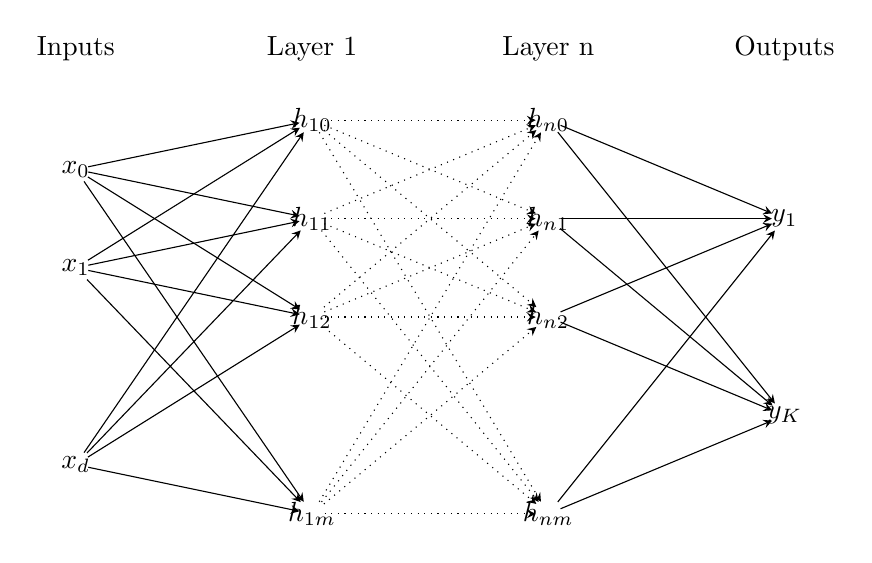
\begin{tikzpicture}[x=1.5cm, y=1.25cm, >=stealth]

\foreach \m/\l [count=\y] in {1,2,missing,3}
  \node [every neuron/.try, neuron \m/.try] (input-\m) at (0,2-\y) {};

\foreach \m [count=\y] in {1,2,3,missing,4}
  \node [every neuron/.try, neuron \m/.try ] (hidden1-\m) at (2,2.5-\y) {};

\foreach \m [count=\y] in {1,2,3,missing,4}
  \node [every neuron/.try, neuron \m/.try ] (hidden2-\m) at (4,2.5-\y) {};

\foreach \m [count=\y] in {1,missing,2}
  \node [every neuron/.try, neuron \m/.try ] (output-\m) at (6,1.5-\y) {};

\foreach \l [count=\i] in {0,1,d}
  \node at (input-\i.center) {$x_{\l}$};

\foreach \l [count=\i] in {0,1,2,m}
  \node at (hidden1-\i.center) {$h_{1\l}$};

  \foreach \l [count=\i] in {0,1,2,m}
  \node at (hidden2-\i.center) {$h_{n\l}$};

\foreach \l [count=\i] in {1,K}
  \node at (output-\i.center) {$y_\l$};

\foreach \i in {1,...,3}
  \foreach \j in {1,...,4}
    \draw [->, shorten <=1pt, shorten >=1pt] (input-\i) -- (hidden1-\j);

\foreach \i in {1,...,4}
  \foreach \j in {1,...,4}
    \draw [dotted, ->, shorten <=1pt, shorten >=1pt] (hidden1-\i) -- (hidden2-\j);

\foreach \i in {1,...,4}
  \foreach \j in {1,...,2}
    \draw [->, shorten <=1pt, shorten >=1pt] (hidden2-\i) -- (output-\j);

\foreach \l [count=\x from 0] in {Inputs, Layer 1, Layer n, Outputs}
  \node [align=center, above] at (\x*2,2) {\l};

\end{tikzpicture}
\caption{A more complex neural network containing an input layer of $d$ nodes corresponding to data of dimensionality $d$, $n$ hidden layers of $m$ hidden units each $h_{ij}$ (where $i$ indexes hidden layer and $j$ indexes a particular unit) and an output layer of $K$ predictive units $y_k$.}
\label{fig:nn}
\end{center}
\end{figure}